\section{Sentinel-1介绍}

从数据获取模式, 产品级别与类型, 数据文件命名规则与组织结构介绍Sentinel-1卫星. 

\subsection{数据获取模式}
Sentinel-1号卫星数据获取模式有 SM(Stripmap), IW(Interferometric Wide swath), EW(Extra Wide swath)和WV(Wave)四种模式, 如图\ref{fig:0201}~所示:
\begin{figure}[htbp]
    \centering
    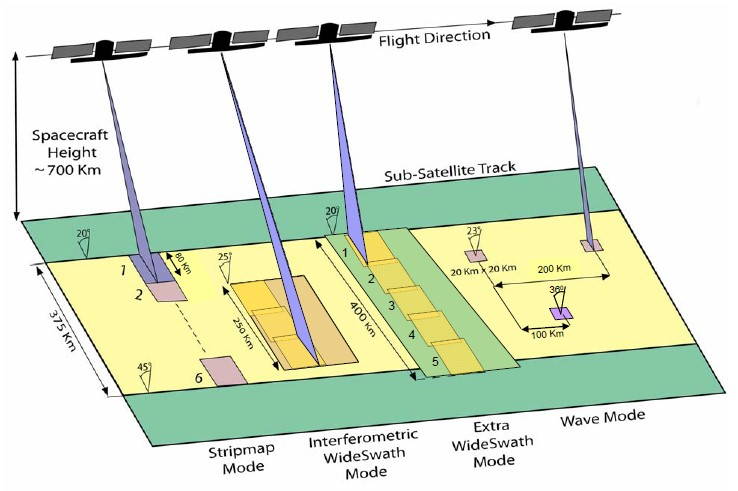
\includegraphics[height=20em]{pic/chap02xx01.jpg}
    \caption{数据获取模式}
    \label{fig:0201}
\end{figure}

\begin{description}
    \item[SM] 一种标准的SAR条形图成像模式, 其中地面区域被连续的脉冲序列照亮, 而天线波束指向一个固定的方位角和仰角. SW模式仅用于小岛屿, 在紧急情况管理等特殊事件时使用.
    \item[IW] IW模式是陆地上的主要采集模式, 满足了大部分业务需求. 它以5米x20米的空间分辨率(单视)获取250公里长的数据.IW模式使用渐进扫描SAR(TOPSAR)地形观测捕获三个子区域. 在TOPSAR技术中, 除了像扫描雷达一样控制波束的范围外, 波束还可以在每个爆发的方位角方向上由后向前进行电子控制, 避免了扇形现象, 并导致整个区域的图像质量均匀.
    \item[EW] 使用TOPSAR成像技术在五个区域获取数据. EW模式以牺牲空间分辨率为代价提供了非常大的区域覆盖.
    \item[WV] 数据是在被称为``小片段''的小型条形地图场景中获取的, 这些场景在轨道沿线每隔100公里定期设置一次. 通过交替获得小点, 以近距离入射角获得一个小点, 而以远距离入射角获得下一个小点. WV多用于海洋观测. 
\end{description}

\subsection{产品级别与类型}

\begin{figure}[htbp]
    \centering
    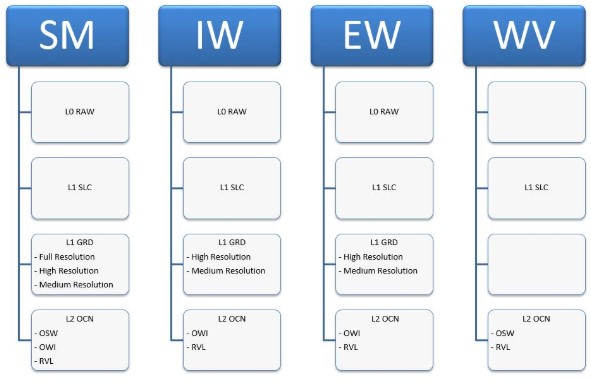
\includegraphics[height=20em]{pic/chap02xx02.jpg}
    \caption{产品级别与类型}
    \label{fig:0202}
\end{figure}

\begin{description}
    \item[Raw] Level-0数据, 特殊情况下使用.
    \item[SLC] Single Look Complex, 已被处理后的一级产品, 能获得相位和振幅信息. 相位信息是时间的函数, 根据相位信息和速度可实现距离的测量, 可用于测距和形变观测.
    \item[GRD] Groud Range Detected , 一级产品, 有多视强度数据, 该强度数据与后向散射系数有关, 可用于土壤水分反演.
    \item[OCN] Ocean, 主要应用与海洋的产品. 
\end{description}
更多关于产品类型的详细参数可见
\hyperref{https://sentinel.esa.int/web/sentinel/user-guides/sentinel-1-sar/resolutions}{}{}{欧空局网站}

\subsection{数据文件命名规则}
\begin{figure}[htbp]
    \centering
    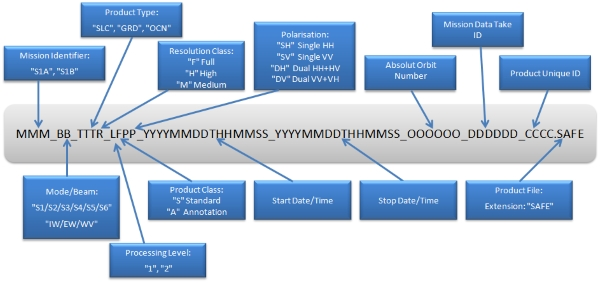
\includegraphics[height=15em]{pic/chap02xx03.jpg}
    \caption{产品级别与类型}
    \label{fig:0203}
\end{figure}

数据文件命名规则如图\ref{fig:0203}~所示.

\begin{description}
    \item[MMM] 卫星的标识码, 如S1A表示哨兵一号A星.
    \item[BB] 数据获取模式, 如IW, EW, MV.
    \item[TTT] 卫星数据类型, 如SLC, GRD, OCN. 
    \item[R] 卫星的分辨率, F为Full Resolution; H为High Resolution, M为Medium Resolution.
    \item[L] 产品等级, 可以为0, 1, 2.
    \item[F] 产品类型, S为Standard, A为Annotation.
    \item[PP] 极化方式, HH, HV, VV, VH
    \item[YY..SS] 第一个为产品开始获取的时间, 第二个为产品获取结束时间
    \item[OOOOOO] 绝对轨道号
    \item[DDDDDD] 任务数据利用标识符
    \item[CCCC] 产品唯一标识码          
\end{description}

\subsection{数据文件组织结构}

一般从欧空局下载的哨兵一号数据, 其文件夹结构如图\ref{fig:0204}~所示:
\begin{figure}[!htbp]
    \centering
    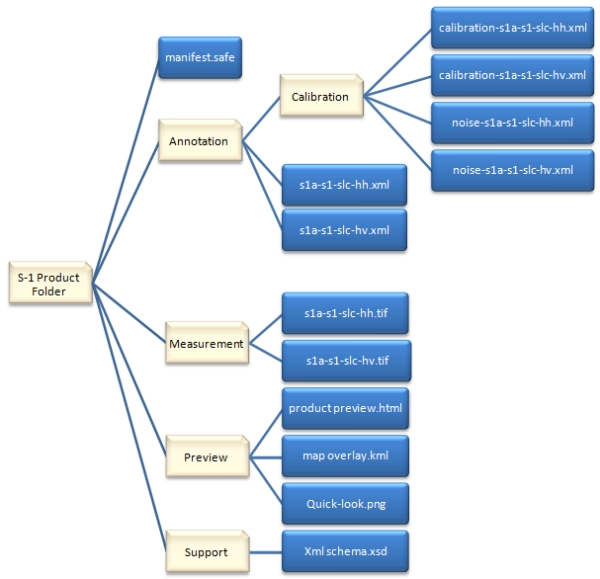
\includegraphics[height=20em]{pic/chap02xx04.jpg}
    \caption{文件组织结构}
    \label{fig:0204}
\end{figure}

\begin{itemize}
    \item 一个manifest.safe文件, 元数据文件, 本质上是一个.xml文件.
    \item 测量数据的子文件夹measurement, 存放的是真正影像数据.tif格式的文件.
    \item 一个包含KML和HTML预览文件的预览子文件夹preview, 存放的是与预览图有关的文件.
    \item 一个注释子文件夹annotation, 存放是卫星拍摄以及定标时的相关数据说明等元数据.
    \item 包含XML模式的支持子文件夹support, 对.xml文件的扩展支持文件.
    \item 此外还有一个关于数据质量的说明文件
\end{itemize}



